\documentclass[10pt]{article}
\usepackage{amsthm}
\usepackage{amsmath}
\usepackage[nochapters]{classicthesis}
\usepackage{pgf, tikz}
\usetikzlibrary{arrows, automata}

\newtheorem{proposition}{Proposition}
\newtheorem{theorem}{Theorem}
\newtheorem{corollary}{Corollary}
\newtheorem{lemma}{Lemma}
\newtheorem{definition}{Definition}
\newtheorem{question}{Question}
\newtheorem{conjecture}{Conjecture}

\newcommand{\defn}[1]{\textit{#1}}
\newcommand{\decprob}[1]{\textsc{#1}}

\begin{document}
\pagestyle{plain}
\title{\rmfamily\normalfont\spacedallcaps{Decision
Problems in Invertible Automata}} \author{\spacedlowsmallcaps{Evan
Bergeron \& Klaus Sutner}} \date{May 5, 2017}

\maketitle

\begin{abstract}
  We consider a variety of decision problems in groups and semigroups
  induced by invertible Mealy machines. Notably, we present proof that
  the automorphism membership problem in decidable in these
  semigroups. In addition, we prove undecidability of a Knapsack
  variant. A discussion of iteration and orbit rationality follows.
\end{abstract}

\tableofcontents

\section{Introduction}
The word problem is a classic group-theoretic decision problem. Given
a finitely generated group $G$, and a word $w$ over the generators
(and their inverses), the word problem asks ``is $w \in G$.'' The word
problem is known to be undecidable in surprisely small classes of
groups - see TODO for background.

The invertible Mealy machines we consider here give rise to a class of
semigroups (and sometimes groups) for which the word problem is
decidable. The computability picture here is rather nuaced,
however. Other important decision problems, among them the conjugacy
problem, and the isomorphism problem are known to be undecidable. (See
TODO and TODO for details).

We present proof that, for the Abelian case, automorphism membership
testing is decidable in this class of semigroups.

\section{Background}
An \defn{automaton} is a formally a triple $(Q, \Sigma, \delta)$,
where $Q$ is some finite state set, $\Sigma$ is a finite alphabet of
\defn{symbols}, and $\delta$ is a transformation on $Q \times \Sigma$.
Automata are typically viewed as directed graphs with vertex set $Q$
and an edge between $u, v$ if $(u, x)\delta = (v, y)$.

An automaton is said to be \defn{synchronous} when $\delta$ outputs
exactly one character for every transition and is called
\defn{invertible} when every state in $Q$ has some bijection $\pi$ on
$\Sigma$ such that $(u, x)\delta = (v, \pi(x))$. A state is a
\defn{copy state} if $\pi$ is the identity permutation and is a
\defn{toggle state} otherwise.

% TODO how to describe clearly?
Each state $q \in Q$ acts on $\Sigma^*$, the set of finite strings
over $\Sigma$. We commonly view $\Sigma^*$ as the infinite
$|\Sigma|$-nary tree, so we may view $q$ as a transformation sending
vertex $w$ to $wq$.

We extend the action of $Q$ on $\Sigma^*$ to words $q = q_1\cdots q_n$
over $Q^+$ by \[ wq = (\cdots((w q_1) q_2)\cdots q_n) \]

We adopt the convention of applying functions from the right here. In
this way, function composition corresponds naturally with
concatenation.

For an automaton $A$, we denote by $S(A)$ the semigroup generated by
$Q$ under composition. $A$ is said to be \defn{commutative} or
\defn{Abelian} when $S(A)$ is Abelian. We write $G(A)$ for the group
generated by the elements of $Q$ and their inverses.

One may also speak about $S(A)$ and $G(A)$ without explicit reference
to an automaton $A$. As such, we call a semigroup $S$ an
\defn{automaton semigroup} if there is some automaton $A$ with
$S \simeq \Sigma(A)$. \defn{Automaton groups} $G$ are similarly
defined.

% Invertible automata have gained popularity in group theory
Invertible automata have recently been usefully applied the group
theory. A classic result here is Grigorchuk's group of intermediate
growth, generated by the 5 state invertible machine shown in figure 1.

% TODO make this not ugly
% TODO make this a figure
\begin{figure}
\begin{center}
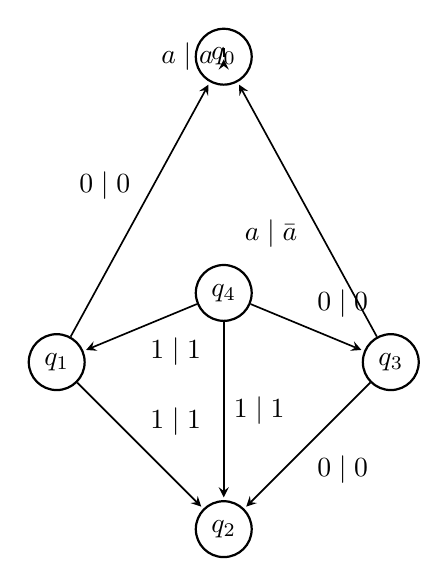
\begin{tikzpicture}[
> = stealth, % arrow head style
shorten > = 1pt, % don't touch arrow head to node
auto,
node distance = 3cm, % distance between nodes
semithick % line style
]
\tikzstyle{every state}=[
draw = black,
thick,
fill = white,
minimum size = 4mm
]
\node[state] (s2) {$q_2$};
\node[state] (s1) [above left of=s2] {$q_1$};
\node[state] (s3) [above right of=s2] {$q_3$};
\node[state] (s4) [above of=s2] {$q_4$};
\node[state] (s0) [above of=s4] {$q_0$};
\path[->] (s0) edge node {$a\mid a$} (s0);
\path[->] (s1) edge node {$0 \mid 0$} (s0);
\path[->] (s3) edge node {$a \mid \bar{a}$} (s0);
\path[->] (s4) edge node {$1 \mid 1$} (s1);
\path[->] (s4) edge node {$0 \mid 0$} (s3);
\path[->] (s4) edge node {$1 \mid 1$} (s2);
\path[->] (s1) edge node {$1 \mid 1$} (s2);
\path[->] (s3) edge node {$0 \mid 0$} (s2);
\end{tikzpicture}
\caption{Grigorchuk's machine}
\end{center}
\end{figure}

% TODO act on the binary tree
% TODO pretty tikz of the tree

\subsection*{Decision Problems}
Automaton semigroups exhibit many interesting and nuanced
computability properties. While it is an easy result that the
\decprob{word problem} is solvable in such semigroups, similar
group-theoretic problems such as the \decprob{conjugacy problem} and
\decprob{finiteness problem} have been shown to be undecidable
(\cite{sunic:conj}, and \cite{gillibert:finite}, respectively).

Various other semigroup theoretic decision problems have recently been
considered for small classes of semigroups by Cain in
\cite{Cain09:dec_prob}. We consider a subset of his distinguished
properties in the automaton semigroup case here.

% TODO
% Example automaton semigroups (and explicit automaton example)
% Recursively presented
% Finitely generated
% Wreath recursions
% Cosets thing

\section{Decidable Abelian Automorphism Membership}

\section{Knapsack is Undecidable for Automaton Semigroups}
We follow a proof strategy similar to \cite{Konig15:knapsack}.

We define the \defn{Knapsack Problem} as follows: given as input
generators $g_1 \ldots g_k$ and a target group element $g$, do there
exist natural numbers $a_1\ldots a_k$ such that
\[ g_1^{a_1} \cdots g_k^{a_K} = g \] We prove that this problem is
undecidable for automaton semigroups by reducing from % to?
Hilbert's tenth problem.

Hilbert's tenth problem asks: ``given a polynomial over the integers
and an integer $a$, do there exist values of the arguments to the
polynomial such that the polynomial evaluated at this point is equal
to $a$?'' It is known that there exist polynomials for which this
problem is undecidable.

We can expand this polynomial into a system of equations - think of a
codegen step in a compiler. Each step is either an addition or a
multiplication. We can take the terms with negative coefficients and
move them to the other side of the equation, so we now have the
equality of two different polynomials, each with positive
coefficients. We can also choose to only substitute in natural numbers
as arguments, by some trick that I don't know. So then we have systems
of equations over the natural numbers.

We can turn each equation into a formulation of the Knapsack problem
for automaton semigroups. It's known that the Heisenberg semigroup is
an automaton group, and there's some equation over the elements of
$H_3$ for multiplication. Same for addition in the natural
numbers. Then we just take the direct product of these groups (the
class of automaton semigroups is closed under direct product). So this
polynomial is equal to $a$ if and only if there exist $a_1 \ldots a_n$
such that each of the individual elements of the direct product
vectors are equal.

\subsection{A group with decidable word problem with submonoid for
  which the IsGroup question is undecidable}

We define the following ambient group: elements of the group represent
states of a turing machine. This turing machine operates on the empty
tape. There is a single halting configuration. In the group, the
element corresponding to the halting configuration is the identity. If
two group elements represent two configurations of the Turing machine
such that one of the configurations can proceed to the other in a
single step, then these two group elements are considered equal.

We have the take care defining the Turing machine, however. We'll
define it to be a \defn{self-verifying} Turing machine. How does this
work? This Turing machine provides some canonical computation, that
is, it proceeds from the start configuration onward, perhaps
halting. However, there are all sorts of configurations that the
Turing machine will never reach. A self-verifying Turing machine will,
at every point, verify that it is along this canonical computation
path. If it finds that it is not, it will transition to some death
state, where it will stay.

This means that, considering the set of all possible configurations of
the Turing machine as a graph, there's a path from the start state
onward (perhaps ending in a halt state) and everything else is just a
star graph transitioning to this death state.

How are these self-verifying Turing machines realized? As the
canonical computation proceeds, a program counter is kept (perhaps to
the left of the tapehead). After every step, the Turing machine will
examine what ``time step'' the computation is currently sitting in. It
will perform the canonical computation for the first $n$ steps. If it
does not wind up where it's configuration says it is, it transitions
to the death state. Otherwise, it continues.

\textit{Claim:} This group has a decidable word problem.

We can verify if one configuration transitions to another in a single
step. So given a word over the generators (that represents a sequence
of TM configurations), we can first go through pairwise, rewriting
these pairs. So I guess chains of consequentive configurations just
become their first state. We can also go through and check to see if
certain configurations lie upon the canonical computational path. So
then everything becomes either the death state or the start state or
the identity? Then we can just check for equality of exponents?

\textit{Claim:} If $s$ is the start configuration of the Turing
machine, it is undecidable whether $\langle s \rangle$ is a group.

Suppose it was decidable. We can, given, a TM, transform it into a
self-verifying version of itself, and then build this group around
it. If the original TM halts, then the submonoid generated by $s$,
(the start state) is just the trivial group. If the original TM hangs,
then $\langle s \rangle$ is the free monoid of rank one. So then being
able to answer the question ``is $\langle s \rangle $ a group'' would
allow us to solve the halting problem.

\subsection{It is decidable if an Abelian automaton semigroup
  generates a group}

Reduces to a system of equations. Abelian automaton semigroups can be
written as a system of matrix equations: residuation is a linear
operation here. We can then also write down the set of matrix
equations for the inverse automaton.\footnote{Interesting to note that
  there's some duality here: if the semigroup of $A$ is a group, then
  so is the semigroup of $A^{-1}$ (and they are equal).}  Exactly what
question do we then ask to verify there is a solution? Something about
asking if the space spanned by the equations for $A$ has any
intersection with $\mathbb{N}^n$.


\subsection{Residuation Fixed Point is Decidable for Abelian automaton
  semigroups}

Take the matrix representing residuation for some word
$w \in \Sigma^*$ and find if it has any eigenvectors in
$\mathbb{N}^n$.

\subsection{Misc}

\begin{proposition}
  In an Abelian, minimal transducer $A$, every state has in-degree at
  most 2.
\end{proposition}
\begin{proof}
  Consider a state $s$. Every parent of $s$ is either a copy or a
  toggle state. If $s$ had two copy state parents, this contradicts
  minimality.

  If $s$ had two toggle state parents $s_1$, $s_2$, then either
  $s = \partial_a s_1 = \partial_a s_2$ or
  $s = \partial_a s_1 = \partial_{\bar{a}} s_2$. Certainly, the first
  case contradicts minimality, since then
  $$ \partial_{\bar{a}} s_1 = \theta \partial_a s_1 = \theta
  \partial_a s_2 = \partial_{\bar{a}} s_2$$ and so $s_1 = s_2$.  For
  the second case, then TODO I have another argument for this.
  $$ \theta \partial_{a} s_1 = \theta \partial_{\bar{a}} s_2 =
  \partial_a s_2 $$ Suppose some state $s$ has in-degree $d \geq
  3$. Then either at least 2 parents are toggles, or at least two are
  copies. If at least 2 are copies,
    \end{proof}

\section{Abelian Automata}

\section{Open Questions}

\begin{itemize}
\item All automaton semigroups are recursively presented. If these
  presentations are regular, or context-free, does that affect the
  soluability of these questions?
\item Having a zero
\item Isomorphism problem
\item Bounded automata, etc
\end{itemize}

\nocite{*}\addtocontents{toc}{\protect\vspace{\beforebibskip}}
\addcontentsline{toc}{section}{\refname} \bibliographystyle{plain}
\bibliography{thesis}
\end{document}
